\subsection{与预层相伴的层}

沿用第 5 号的记号，我们把 \(\widetilde{\mathcal{F}}\) 称为与预层 \(\mathcal{F}\) 相伴的层，并用 \(\widetilde{\mathcal{F}}\) 表示层 \(\underline{\mathcal{L}}(\mathrm{B};\mathrm{E}_{\mathcal{F}})\)，即平展 B-空间 \(\mathrm{E}_{\mathcal{F}}\) （与预层 \(\mathcal{F}\) 相伴的）的连续截面所成的层。对每个开集 \(\mathrm{U}\in\mathcal{B}\)，用 \(\sigma_{\mathcal{F}}(\mathrm{U})\colon\mathcal{F}(\mathrm{U})\to\widetilde{\mathcal{F}}(\mathrm{U})\) 表示把 \(s\in\mathcal{F}(\mathrm{U})\) 映为连续截面 \(\sigma_{\mathcal{F}}(\mathrm{U},s)\colon x\mapsto[\mathrm{U},s,x]\) （\(\mathrm{E}_{\mathcal{F}}\) 在 U 上的）的映射。由等价关系 \(\mathrm{R}_{\mathcal{F}}\) 的定义，族 \(\sigma_{\mathcal{F}}=(\sigma_{\mathcal{F}}(\mathrm{U}))_{\mathrm{U}\in\mathcal{B}}\) 是从 \(\mathcal{F}\) 到预层 \(\widetilde{\mathcal{F}}|\mathcal{B}\) 中的预层的态射。态射 \(\sigma_{\mathcal{F}}\) 称为从 \(\mathcal{F}\) 到 \(\widetilde{\mathcal{F}}|\mathcal{B}\) 中的典范态射。

用 \(j_{\mathcal{F}} \colon \mathrm{E}_{\mathcal{F}} \to \mathrm{E}_{\widetilde{\mathcal{F}}}\) 表示由典范 B-同构 \(\mathrm{E}_{\widetilde{\mathcal{F}}|\mathcal{B}} \to \mathrm{E}_{\widetilde{\mathcal{F}}}\) （I, p. 51）与 B-态射 \(\mathrm{E}(\sigma_{\mathcal{F}}) \colon \mathrm{E}_{\mathcal{F}} \to \mathrm{E}_{\widetilde{\mathcal{F}}|\mathcal{B}}\) 合成的 B-态射。再用 \(e_{\mathcal{F}} \colon \mathrm{E}_{\widetilde{\mathcal{F}}} \to \mathrm{E}_{\mathcal{F}}\) 表示典范 B-同构 (I, p. 52, 例 2)。

命题 2. --- 映射 \(j_{\mathcal{F}}\) 是 \(e_{\mathcal{F}}\) 的逆 B-同构。

对 \(\mathrm{U}\in \mathcal{B}\)、\(s\in \mathcal{F}(\mathrm{U})\) 与 \(x\in \mathrm{U}\)，由 \(j_{\mathcal{F}}\) 的定义，我们有：

\[
j _ {\mathcal {F}} ([ \mathrm{U}, s, x ]) = [ \mathrm{U}, \sigma_ {\mathcal {F}} (\mathrm{U}, s), x ],
\]

由此得 \(e_{\mathcal{F}}(j_{\mathcal{F}}([U,s,x])) = \sigma_{\mathcal{F}}(U,s)(x) = [U,s,x]\)。这就证明了该命题。

推论. --- 对每个 \(a \in B\)，映射 \((\sigma_{\mathcal{F}})_{a}\) : \(F_{a} \to \widetilde{F}_{a}\) 是双射。

由于 \(j_{F}\) 是 B-同构，故 \(\mathrm{E}(\sigma_{\mathcal{F}})\) 亦然，而 \((\sigma_{\mathcal{F}})_{a}\) 是在 a 处过渡到纤维而得到的。

设 \(\mathcal{G}\) 为 B 上相对于 \(\mathcal{B}\) 的一个预层，\(\varphi\colon\mathcal{F}\to\mathcal{G}\) 为预层的一个态射。我们用 \(\widetilde{\varphi}\colon\widetilde{\mathcal{F}}\to\widetilde{\mathcal{G}}\) 表示层的态射 \(\underline{\mathcal{L}}_{\mathrm{E}(\varphi)}\) （I, p. 48, 例 1），其中 \(\mathrm{E}(\varphi)\colon\mathrm{E}_{\mathcal{F}}\to\mathrm{E}_{\mathcal{G}}\) 是与 \(\varphi\) 相伴的 B-态射。对每个开集 \(\mathrm{U}\in\mathcal{B}\) 与每个 \(s\in\mathcal{F}(\mathrm{U})\)，由定义我们有

\[
\widetilde {\varphi} _ {\mathrm{U}} (\sigma_ {\mathcal {F}} (\mathrm{U}, s)) = \mathrm{E} (\varphi) \circ \sigma_ {\mathcal {F}} (\mathrm{U}, s) = \sigma_ {\mathcal {G}} (\mathrm{U}, \varphi_ {\mathrm{U}} (s)).
\]

于是我们有：

\[
\widetilde {\varphi} _ {\mathrm{U}} \circ \sigma_ {\mathcal {F}} (\mathrm{U}) = \sigma_ {\mathcal {G}} (\mathrm{U}) \circ \varphi_ {\mathrm{U}}, \quad \text {   for   every   } \mathrm{U} \in \mathcal {B}.\tag{1}
\]

换言之：

\[
\widetilde {\varphi} \mid \mathcal {B} \circ \sigma_ {\mathcal {F}} = \sigma_ {\mathcal {G}} \circ \varphi .\tag{2}
\]

命题 3. --- 设 B 为拓扑空间，\(\mathcal{B}\) 为 B 的拓扑的一个基，\(\mathcal{F} = (\mathcal{F}(\mathrm{U}), f_{\mathrm{UV}})\) 为 B 上相对于 \(\mathcal{B}\) 的一个预层，\(\widetilde{\mathcal{F}}\) 为相伴层，\(\sigma_{\mathcal{F}}: \mathcal{F} \to \widetilde{\mathcal{F}} \mid \mathcal{B}\) 为典范态射。给定 B 上的一个层 \(\mathcal{G} = (\mathcal{G}(\mathrm{U}), g_{\mathrm{UV}})\) 与预层的一个态射 \(\varphi: \mathcal{F} \to \mathcal{G} \mid \mathcal{B}\)，存在唯一的层的态射 \(\psi: \widetilde{\mathcal{F}} \to \mathcal{G}\) 满足 \(\psi \mid \mathcal{B} \circ \sigma_{\mathcal{F}} = \varphi\)。

引理. --- 设 U 为 B 的一个开子集，\(s\colon U \to E_{\mathcal{F}}\) 为 \(E_{\mathcal{F}}\) 在 U 上的一个连续截面。对 U 的每个点 a，存在开集 \(V \in \mathcal{B}\) 满足 \(a \in V\) 与 \(V \subset U\)，以及元素 v （\(\mathcal{F}(V)\) 的）满足 \(s \mid V = \sigma_{\mathcal{F}}(V, v)\)。

设 \(a \in \mathrm{U}\)。由空间 \(\mathrm{E}_{\mathcal{F}}\) 的定义，存在开集 \(\mathrm{V}' \in \mathcal{B}\) 满足 \(a \in \mathrm{V}'\)，以及元素 \(t\) （\(\mathcal{F}(\mathrm{V}')\) 的）满足 \(s(a) = [\mathrm{V}', t, a]\)。于是 \(s\) 与 \(\sigma_{\mathcal{F}}(\mathrm{V}', t)\) 由限制诱导出 \(\mathrm{E}_{\mathcal{F}}\) 在 \(\mathrm{V}' \cap \mathrm{U}\) 上的两个连续截面，二者在点 \(a\) 处相等。由 I, p. 34 的 prop. 11, b)，存在 \(a\) 的一个开邻域 V，它含于 \(\mathrm{V}' \cap \mathrm{U}\) 且属于 \(\mathcal{B}\)，使得 \(s\) 与 \(\sigma_{\mathcal{F}}(\mathrm{V}', t)\) 在 V 的每一点处相合。若令 \(v = f_{\mathrm{VV}'}(t)\)，则确有 \(s \mid \mathrm{V} = \sigma_{\mathcal{F}}(\mathrm{V}, v)\)。

我们来证明该命题。对 B 的每个开集 U 与每个截面 \(s \in \widetilde{\mathcal{F}}(\mathrm{U})\)，用 \(\mathrm{D}(\mathrm{U}, s)\) 表示对 \((\mathrm{V}, v)\) （满足 \(V \in \mathcal{B}\)、\(V \subset U\)、\(v \in \mathcal{F}(\mathrm{V})\) 且 \(s | V = \sigma_{\mathcal{F}}(V, v)\) 者）所成的集。由引理，这些开集 V 构成 U 的一个覆盖。

若存在态射 \(\psi\colon\mathcal{F}\to\mathcal{G}\) 满足 \(\psi\mid\mathcal{B}\circ\sigma_{\mathcal{F}}=\varphi\)，则对 B 的每个开集 U、每个截面 \(s\in\widetilde{\mathcal{F}}(\mathrm{U})\) 与每个对 \((\mathrm{V},v)\in\mathrm{D}(\mathrm{U},s)\)，我们有 \(g_{\mathrm{VU}}(\psi_{\mathrm{U}}(s))=\psi_{\mathrm{V}}(s\mid\mathrm{V})=\varphi_{\mathrm{V}}(v)\)。这便证明了 \(\psi\) 的唯一性，依据是层的性质 \((\mathrm{F}_{1})\)。

设 U 为 B 的一个开集，s 为 \(\widetilde{\mathcal{F}}(\mathrm{U})\) 的一个元素。设 \((\mathrm{V},v)\) 与 \((\mathrm{V}^{\prime},v^{\prime})\) 为 \(\mathrm{D}(\mathrm{U},s)\) 的元素。我们有 \(s(a)=[\mathrm{V},v,a]=[\mathrm{V}^{\prime},v^{\prime},a]\) 对每一点 \(a\in V\cap V^{\prime}\) 成立。因此，存在对 \((\mathrm{W},w)\in\mathrm{D}(\mathrm{V}\cap\mathrm{V}^{\prime},s)\) 满足 \(a\in W\) 与 \(f_{\mathrm{WV}}(v)=f_{\mathrm{WV}}(v^{\prime})=w\)。于是有

\[
g _ {\mathrm{W} (\mathrm{V} \cap \mathrm{V} ^ {\prime})} \circ g _ {(\mathrm{V} \cap \mathrm{V} ^ {\prime}) \mathrm{V}} (\varphi_ {\mathrm{V}} (v)) = g _ {\mathrm{WV}} (\varphi_ {\mathrm{V}} (v)) = \varphi_ {\mathrm{W}} (f _ {\mathrm{WV}} (v)) = \varphi_ {\mathrm{W}} (w)
\]

同样，

\[
g _ {\mathrm{W} (\mathrm{V} \cap \mathrm{V} ^ {\prime})} \circ g _ {(\mathrm{V} \cap \mathrm{V} ^ {\prime}) \mathrm{V} ^ {\prime}} (\varphi_ {\mathrm{V} ^ {\prime}} (v ^ {\prime})) = \varphi_ {\mathrm{W}} (w),
\]

从而

\[
g _ {\mathrm{W} (\mathrm{V} \cap \mathrm{V} ^ {\prime})} \circ g _ {(\mathrm{V} \cap \mathrm{V} ^ {\prime}) \mathrm{V}} (\varphi_ {\mathrm{V}} (v)) = g _ {\mathrm{W} (\mathrm{V} \cap \mathrm{V} ^ {\prime})} \circ g _ {(\mathrm{V} \cap \mathrm{V} ^ {\prime}) \mathrm{V} ^ {\prime}} (\varphi_ {\mathrm{V} ^ {\prime}} (v ^ {\prime})).
\]

于是由层的性质 (F \(_{1}\) )，我们有

\[
g _ {(\mathrm{V} \cap \mathrm{V} ^ {\prime}) \mathrm{V}} (\varphi_ {\mathrm{V}} (v)) = g _ {(\mathrm{V} \cap \mathrm{V} ^ {\prime}) \mathrm{V} ^ {\prime}} (\varphi_ {\mathrm{V} ^ {\prime}} (v ^ {\prime})).
\]

由层的性质 \((\mathrm{F}_{1})\) 与 \((\mathrm{F}_{2})\)，存在唯一的元素 \(\psi_{\mathrm{U}}(s) \in \mathcal{G}(\mathrm{U})\) 使得：

\[
g _ {\mathrm{VU}} \left(\psi_ {\mathrm{U}} (s)\right) = \varphi_ {\mathrm{V}} (v) \quad \text {   for   every   } (\mathrm{V}, v) \in \mathrm{D} (\mathrm{U}, s).\tag{3}
\]

设 \(\psi_{\mathrm{U}}\colon \widetilde{\mathcal{F}} (\mathrm{U})\to \mathcal{G}(\mathrm{U})\) 为这样定义的映射。由 (3) 立即得出：族 \(\psi = (\psi_{\mathrm{U}})\) 是层的态射，并且有 \(\varphi_{\mathrm{V}} = \psi_{\mathrm{V}}\circ \sigma_{\mathcal{F}}(\mathrm{V})\) 对一切 \(\mathrm{V}\in \mathcal{B}\) 成立。

推论 1. --- 设 B 为拓扑空间，\(\mathcal{F}\) 为 B 上的一个预层，\(\widetilde{\mathcal{F}}\) 为相伴层，\(\sigma_{\mathcal{F}}\colon \mathcal{F} \to \widetilde{\mathcal{F}}\) 为典范态射。为使 \(\mathcal{F}\) 是一个层，必须且只需 \(\sigma_{\mathcal{F}}\) 是同构。

若 \(\sigma_{\mathcal{F}}\) 是同构，则 \(\mathcal{F}\) 是层。反之，若 \(\mathcal{F}\) 是层，则由命题 3 存在一个态射 \(\varphi: \widetilde{\mathcal{F}} \to \mathcal{F}\) 满足 \(\varphi \circ \sigma_{\mathcal{F}} = \operatorname{Id}_{\mathcal{F}}\)。由于 \(\operatorname{Id}_{\widetilde{\mathcal{F}}}\) 是唯一的态射 \(\psi: \widetilde{\mathcal{F}} \to \widetilde{\mathcal{F}}\) （满足 \(\psi \circ \sigma_{\mathcal{F}} = \sigma_{\mathcal{F}}\) 者），故有 \(\sigma_{\mathcal{F}} \circ \varphi = \operatorname{Id}_{\widetilde{\mathcal{F}}}\)。

注. --- 设 B 为拓扑空间，\(\mathcal{F}\) 为 B 上的一个预层，\(\mathcal{G}\) 为 B 上的一个层，\(\varphi\colon\mathcal{F}\to\mathcal{G}\) 为预层的一个态射。典范态射 \(\sigma_{\mathcal{G}}\colon\mathcal{G}\to\widetilde{\mathcal{G}}\) 依推论 1 是同构。于是由 I, p. 54 的关系式 (2)，唯一的态射 \(\psi\colon\widetilde{\mathcal{F}}\to\mathcal{G}\) （满足 \(\psi\circ\sigma_{\mathcal{F}}=\varphi\) 者）就是 \(\sigma_{\mathcal{G}}^{-1}\circ\widetilde{\varphi}\)。

推论 2. --- 设 B 为拓扑空间，F 与 G 为 B 上的层，φ 为从 F 到 G 的层的一个态射。下列断言等价：

\begin{enumerate}
\def\labelenumi{(\roman{enumi})}
\item
  \(\varphi\) 是同构；
\item
  存在 B 的拓扑的一个基 \(\mathcal{B}\)，使得对每个 \(\mathrm{U} \in \mathcal{B}\)，映射 \(\varphi_{\mathrm{U}}\) 是双射；
\item
  对 B 的每一点 \(a\)，映射 \(\varphi_{a}\) 是从茎 \(\mathcal{F}_{a}\) 到茎 \(\mathcal{G}_{a}\) 上的一个双射。
\end{enumerate}

蕴涵 (i)⇒(ii) 是显然的。

(ii)⇒(iii)：考察交换图 (I, p. 51)

\[
\begin{array}{c} \mathrm{E} _ {\mathcal {F} | \mathcal {B}} \xrightarrow {\mathrm{E} (\varphi | \mathcal {B})} \mathrm{E} _ {\mathcal {G} | \mathcal {B}} \\ \Big \downarrow \qquad \qquad \qquad \qquad \qquad \Big \downarrow \\ \mathrm{E} _ {\mathcal {F}} \xrightarrow {\mathrm{E} (\varphi)} \mathrm{E} _ {\mathcal {G}}, \end{array}
\]

其中竖直箭头是典范 B-同构。若条件 (ii) 满足，则 \(\mathrm{E}(\varphi \mid \mathcal{B})\) 是 B-同构，从而 \(\mathrm{E}(\varphi)\) 亦是。诸映射 \(\varphi_{a}\) 由 \(\mathrm{E}(\varphi)\) 过渡到纤维而得，从而都是双射。

(iii)⇒(i)：在假设 (iii) 之下，映射 \(\mathrm{E}(\varphi)\colon E_{\mathcal{F}} \to E_{\mathcal{G}}\) 是平展空间间的一个双射 B-态射，因而是 B-同构 (I, p. 30, prop. 6 的 cor. 2)。从而态射 \(\widetilde{\mathcal{F}}\to\widetilde{\mathcal{G}}\) 是同构。由于 \(\mathcal{F}\) 与 \(\mathcal{G}\) 都是层，典范态射 \(\sigma_{\mathcal{F}}\colon\mathcal{F}\to\widetilde{\mathcal{F}}\) 与 \(\sigma_{\mathcal{G}}\colon\mathcal{G}\to\widetilde{\mathcal{G}}\) 都是同构（推论 1），且有 \(\widetilde{\varphi}\circ\sigma_{\mathcal{F}}=\sigma_{\mathcal{G}}\circ\varphi\) （I, p. 54, 关系式 (2)）；因此 \(\varphi\) 是同构。

附记. --- 设 B 为一个拓扑空间。对 B 上的每个层 \(\mathcal{F}\)，有一个平展 B-空间 \(\mathrm{E}_{\mathcal{F}}\) 与之相伴随（I, p. 50, def. 4）。对每个平展 B-空间 T，有由其连续截面在 B 上所成的层 \(\underline{\mathcal{L}}(\mathrm{T})\) 与之相伴随（I, p. 45, 例 3）。存在层的典范同构 \(\sigma_{\mathcal{F}}\colon \mathcal{F}\to \underline{\mathcal{L}}(\mathrm{E}_{\mathcal{F}})\) （I, p. 55, cor. 1）与平展 B-空间的典范同构 \(e_{\mathrm{T}}\colon \mathrm{E}_{\underline{\mathcal{L}}(\mathrm{T})}\to \mathrm{T}\) （I, p. 52, 例 2）。

对 B 上的每一对层 \((\mathcal{F},\mathcal{G})\)，我们已定义过 (I, p. 50) 一个映射 \(\varphi\mapsto\mathrm{E}(\varphi)\)，它把从 \(\mathcal{F}\) 到 \(\mathcal{G}\) 的层态射所成的集映为从 \(E_{F}\) 到 \(E_{G}\) 的 B-态射所成的集。我们有关系式

\[
\mathrm{E} (\mathrm{Id} _ {\mathcal {F}}) = \mathrm{Id} _ {\mathrm{E} _ {\mathcal {F}}}, \qquad \mathrm{E} (\psi \circ \varphi) = \mathrm{E} (\psi) \circ \mathrm{E} (\varphi).
\]

对平展 B-空间的每一对 (T, U)，已定义过 (I, p. 48, 例 1) 一个映射 \(f \mapsto \underline{\mathcal{L}}(f)\)，它把从 T 到 U 的 B-态射所成的集映为从 \(\underline{\mathcal{L}}(T)\) 到 \(\underline{\mathcal{L}}(U)\) 的层态射所成的集。我们有关系式

\[
\underline {{\mathcal {S}}} (\mathrm{Id} _ {\mathrm{T}}) = \mathrm{Id} _ {\underline {{\mathcal {S}}} (\mathrm{T})}, \qquad \underline {{\mathcal {S}}} (g \circ f) = \underline {{\mathcal {S}}} (g) \circ \underline {{\mathcal {S}}} (f).
\]

采用前面的记号，下列图是交换的：

\begin{enumerate}
\def\labelenumi{(\arabic{enumi})}
\setcounter{enumi}{3}
\tightlist
\item
\item
  \pandocbounded{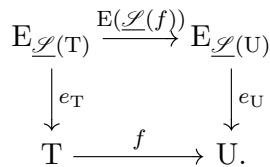
\includegraphics[keepaspectratio]{images/part001_16180f76.jpg}}
\end{enumerate}

对第一个图，这由 I, p. 54 的公式 (2) 得出；对第二个图，它是定义的直接推论。由此推出：对 B 上的每一对层 \((\mathcal{F},\mathcal{G})\) 与平展 B-空间的每一对 (T,U)，上面所考虑的映射 \(\varphi\mapsto\mathrm{E}(\varphi)\) 与 \(f\mapsto\underline{\mathcal{L}}(f)\) 都是双射。

这些结果使得我们能从关于 B 上的层的一个命题推出关于平展 B-空间的一个命题，反之亦然。

